%
% Scott Percic
%
\documentclass[12pt,fullpage]{article}
\usepackage{fullpage}
\usepackage{psfrag}                                          % LaTeX graphics tool
\usepackage{pslatex}                                         % avoids the default cmr font
\usepackage{graphicx}                                        % graphics package 
\usepackage{epsfig}                                          % figures
\usepackage{hyperref}
\usepackage{color}

\begin{document}

\noindent
{\bf Beta distribution} (from \color{blue}\url{http://www.math.wm.edu/~leemis/chart/UDR/UDR.html}\color{black})

{\begin{figure}[b!]
\begin{center}
\psfrag{lab1}{$\beta = 0.5$}
\psfrag{lab2}{$\gamma = 0.5$}
\psfrag{lab3}{$\gamma = 1$}
\psfrag{lab4}{$\gamma = 2$}
\psfrag{lab5}{$\beta = 1$}
\psfrag{lab6}{$\beta = 2$}
\includegraphics[width=6.0in]{BetaPlot.ps}
\end{center}
\end{figure}}

\noindent
The shorthand $X \sim {\rm beta}(\beta, \gamma)$ is used to indicate that the
random variable $X$ has the beta distribution with parameters beta and gamma.
A beta random variable $X$ with positive shape parameters $\beta$~and~$\gamma$ has probability density function 
$$
f(x) =\frac{\Gamma(\beta + \gamma) x ^ {\kern 0.08 em \beta - 1} (1 - x) ^ {\gamma - 1}}{\Gamma(\beta)\Gamma(\gamma)} \qquad \qquad 0<x<1.
$$
The beta distribution is used for modeling random variables that lie between~0 and~1 (for example,
percentages or interest rates) and as a prior distribution (for example, the beta--binomial
distribution).
Probability density functions with various values of the parameters are illustrated below.

The cumulative distribution function on
the support of $X$ is
$$
F(x) = P(X \le x) = I_{x} (\beta, \gamma) \qquad \qquad 0<x<1,
$$
where $I_x$ is the regularized incomplete beta function:
$$
I_{x} (a,b) = \frac{B_x(a, b)}{B(a, b)},
$$
where the beta function is
$$
B(a, b) = \frac{\Gamma(a) \Gamma(b)}{\Gamma(a + b)}
$$
and the incomplete beta function is
$$
B_x(a, b) = \int_0^x t ^ {a - 1} (1 - t) ^ {b - 1} dt.
$$
For integer values of $a$ and $b$, the regularized incomplete beta function can be
computed via
$$
I_{x} (a,b) = \sum_{j = a} ^ {a + b - 1} \frac{(a + b - 1) ! }{j ! (a + b - 1 - j) ! }
\kern 0.08 em x ^ {j}(1 - x) ^ {a + b - 1 - j}.
$$
The survivor function on the support of $X$ is
$$
S(x) = P(X \ge x) = 1- I_{x} (\beta, \gamma) \qquad \qquad 0<x<1.
$$
The hazard function on the support of $X$ is
$$
h(x) = \frac{f(x)}{S(x)} = \frac{\Gamma(\beta + \gamma) x ^ {\beta - 1}(1 - x) ^ {\gamma - 1}}{(1 - I_{x} (\beta, \gamma)) \Gamma(\beta) \Gamma(\gamma)} \qquad \qquad 0<x<1.
$$
The cumulative hazard function and the inverse distribution function are mathematically intractable.
The median of $X$ is found by solving 
$$
I_m(\beta, \gamma) = 0.5
$$
for $m$.
%  $$
%  I \kern 0.08 em _{0.5}^{-1}(\beta,\gamma)
%  $$
%  The moment generating function of $X$ is
%  $$
%  M(t) = 1 + \sum_{k = 1} ^ {\infty} \left( \prod_{r = 0} ^ {k - 1}\frac{\beta + r}{\beta + \gamma + r}\right) \frac{t ^ {k}} {k !}\qquad \qquad t < \lambda.
%  $$
%  The characteristic function of $X$ is
%  $$
%  \phi(t) = E\left[ e ^ {\kern 0.08 em itX} \right] = _{1}F_{1}(\beta; \beta + \gamma; it) \qquad \qquad t < \lambda.
%  $$
The population mean, variance, skewness, and kurtosis of $X$ are
$$
E[X] = \frac{\beta} {\beta + \gamma} 
$$
$$
V[X] = \frac{\beta \gamma}{(\beta + \gamma) ^ {2} (\beta + \gamma + 1)} 
$$
$$
E\left[ \left( \frac{X - \mu}{\sigma} \right) ^ {\kern -0.08 em 3} \right] =\frac{2(\gamma-\beta)\sqrt{1+\beta + \gamma}}{\sqrt{\beta \kern 0.08 em \gamma}\kern 0.08 em (\beta+\gamma+2)}
$$
$$
E\left[ \left( \frac{X - \mu}{\sigma} \right) ^ {\kern -0.08 em 4} \right] =  
\frac {3 \left( \beta^2 \gamma + \beta \gamma ^ 2 - 2 \beta \gamma + 2 \beta ^ 2 + 2 \gamma ^ 2  \right) \left( 1+ \beta + \gamma \right) }
{\beta \kern 0.08 em \gamma \kern 0.08 em (\beta+\gamma+2)(\beta+\gamma+3)}
$$
% $$
% E\left[ \left( \frac{X - \mu}{\sigma} \right) ^ {\kern -0.08 em 4} \right] =  \frac{6 \left[\beta^{3}+\beta^{2}(1-2\gamma)+\gamma^{\kern 0.08 em 2}(1+\gamma)-2\kern 0.08 em \beta \kern 0.08 em \gamma \kern 0.08 em (2+\gamma)\right]}{\beta \kern 0.08 em \gamma \kern 0.08 em (\beta+\gamma+2)(\beta+\gamma+3)}.
% $$

\newpage

\vspace{0.1in}
\noindent
{\bf APPL verification:}
The APPL statements
\begin{verbatim}
X := BetaRV(beta, g);
CDF(X);
SF(X);
HF(X);
IDF(X);
Mean(X);
Variance(X);
Skewness(X);
Kurtosis(X);
\end{verbatim}
verify the cumulative distribution function, survivor function, hazard function,
population mean, variance, skewness, and kurtosis.
Note the use of {\tt g} as a parameter instead of {\tt gamma} due to APPL error.
\end{document}
